\documentclass[tikz]{standalone}
\usepackage{tikz}
\usetikzlibrary{
	shapes,
	snakes,
	calc,
	decorations,
	decorations.markings,
	decorations.text,
	decorations.pathreplacing}
	
\begin{document}
	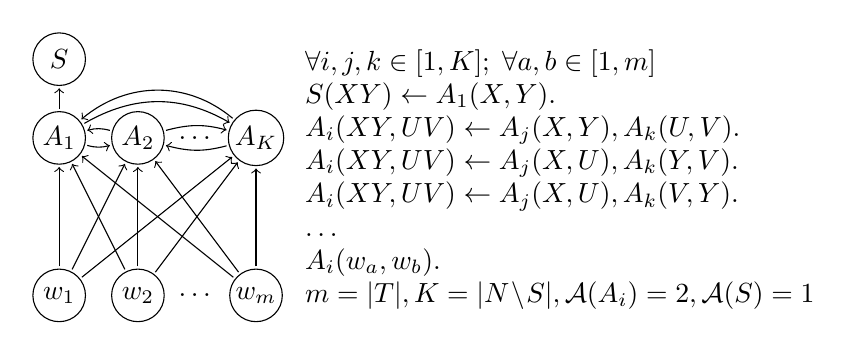
\begin{tikzpicture}[scale=1,every text node part/.style={align=left}]
		\tikzstyle{vertex}=[circle,draw,minimum size=19pt,
							inner sep=1pt, outer sep=1pt]
    	
		 \clip (0.6,-0.4) rectangle (10.6,3.4);
		
    	% S
        \node[vertex] (S) at (1,3) {$S$};
    
    	% As
    	\foreach \name/\x in {A_1/1, A_2/2, A_K/3.5}
       		\node[vertex] (\name) at (\x,2) {$\name$};
    	\node (Adots) at (2.75 ,2) {\ldots};
    	
        % ws
        \foreach \name/\x in {w_1/1, w_2/2, w_m/3.5}
        	\node[vertex] (\name) at (\x,0) {$\name$};
        \node (wdots) at (2.75 ,0) {\ldots};
        
        % edges
        \draw [<-] (S) -- (A_1);
        
        \foreach \wname in {w_1, w_2, w_m}
            \foreach \aname in {A_1, A_2, A_K}
                \draw [->] (\wname) -- (\aname);
                
        \draw [->] (A_1) to [out=345,in=195] (A_2);
        \draw [->] (A_1) to [out=30,in=150] (A_K);
        \draw [->] (A_2) to [out=165,in=15] (A_1);
        \draw [->] (A_2) to [out=15,in=165] (A_K);
        \draw [->] (A_K) to [out=140,in=40] (A_1);
        \draw [->] (A_K) to [out=195,in=345](A_2);
        
        
        \node [anchor=north west] (desc) at (4,3.25) {$\forall i,j,k \in [1,K];\; \forall a,b \in [1,m]$\\$S(XY) \leftarrow A_1(X,Y).$\\$A_i(XY,UV) \leftarrow A_j(X,Y), A_k(U,V).$\\$A_i(XY,UV) \leftarrow A_j(X,U), A_k(Y,V).$\\$A_i(XY,UV) \leftarrow A_j(X,U), A_k(V,Y).$\\$\dots$\\$A_i(w_a,w_b).$\\$m = |T|,K = |N\!\setminus\!S|,\mathcal{A}(A_i) = 2,\mathcal{A}(S) = 1$};
        
	\end{tikzpicture}
\end{document}
